% !TEX encoding = UTF-8 Unicode
\documentclass{beamer}

\usepackage{color}
\usepackage{fancyvrb}
\usepackage{gensymb}
\usepackage{hyperref}
\usepackage{textcomp}
\usepackage{tikz}

\usetikzlibrary{arrows,positioning,shapes,shapes.multipart} 
\tikzstyle{every picture}+=[remember picture]

\definecolor{mygreen}{rgb}{0.88,0.95,0.88}

\usetheme{Warsaw}

\title[Data Visualization with R - R Markdown tutorial]{Data Visualization with R \\ R Markdown tutorial}
\author{Ariane Ducellier}
\date{University of Washington - Fall 2023}

\begin{document}

	\begin{frame}
		\titlepage
	\end{frame}

	\begin{frame}
		\frametitle{Installing R and RStudio}

		Install the latest version of R from the CRAN website: \href{https://cran.r-project.org/}{https://cran.r-project.org/}

		\vspace{2em}

		Install the latest version of RStudio from \href{https://posit.co/download/rstudio-desktop/}{https://posit.co/download/rstudio-desktop/}

		\vspace{2em}

		Open RStudio and Go to File $>$ New File $>$ R Markdown
		
	\end{frame}

	\begin{frame}
		\frametitle{RStudio interface}

		\centering
		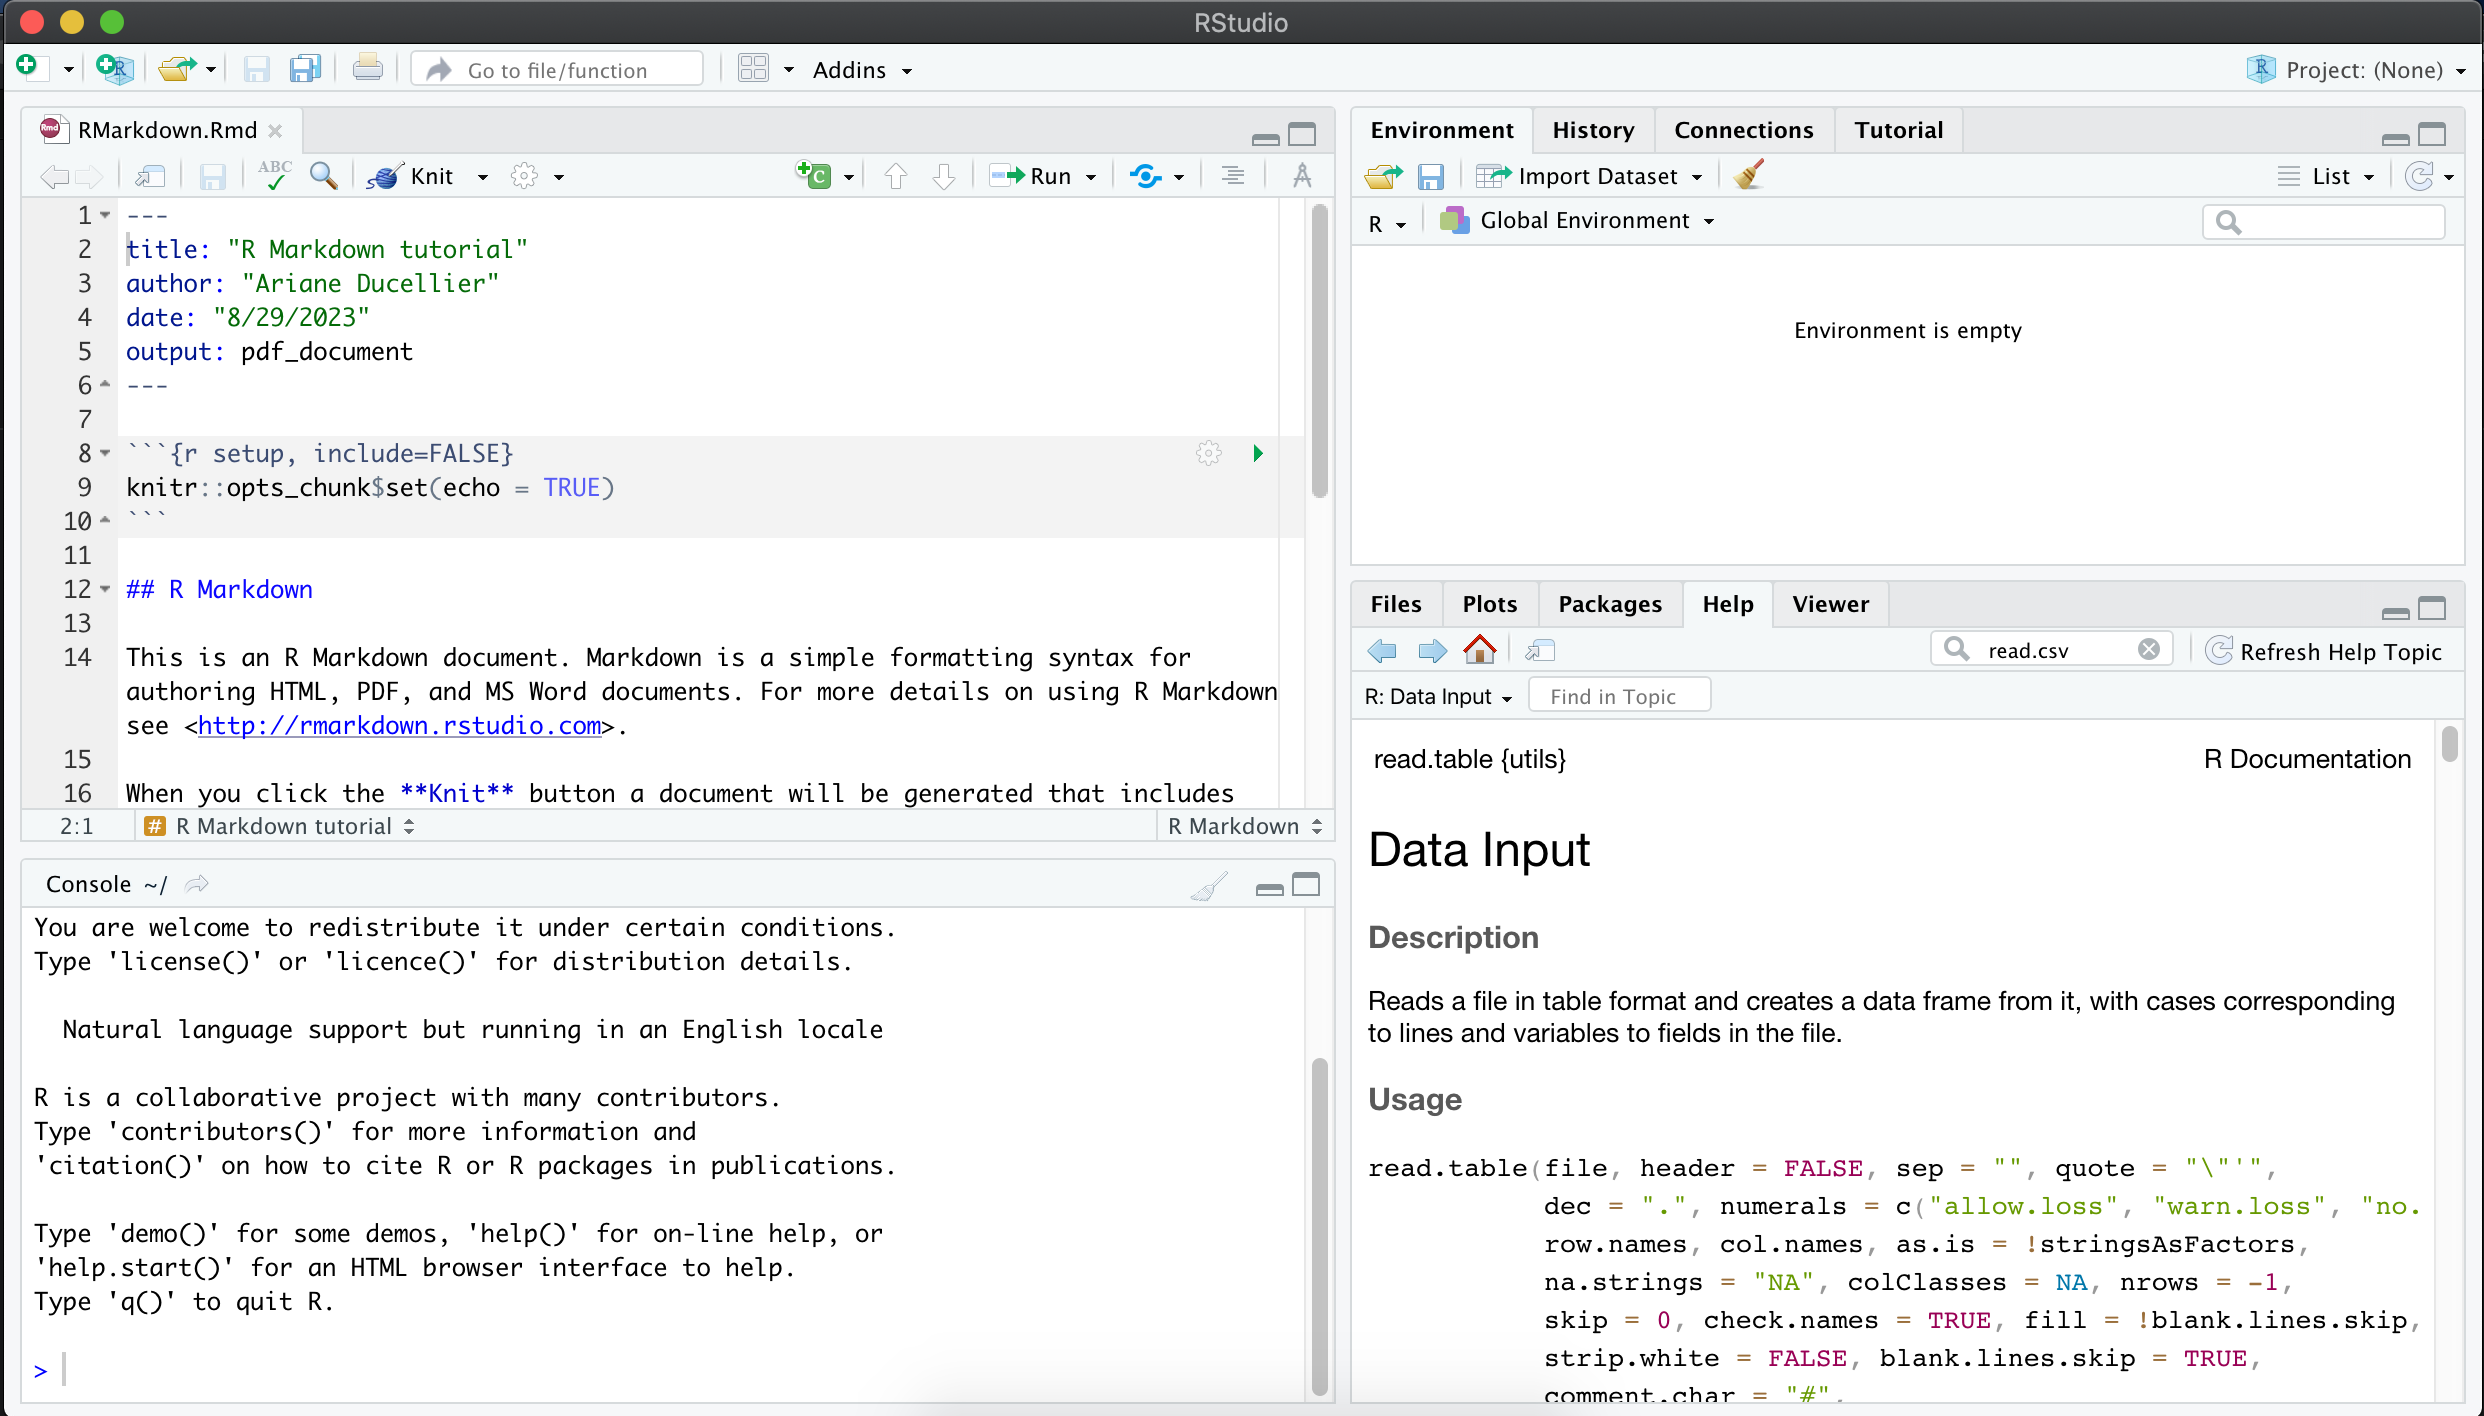
\includegraphics[trim={0cm 0cm 0cm 0cm}, clip, width=11cm]{RMarkdown.png}
		
	\end{frame}

	\begin{frame}[fragile]
		\frametitle{Rmd file structure}

		YAML header:

		\begin{exampleblock}{}
		\begin{BVerbatim}
		---
		title: "R Markdown tutorial"
		author: "Ariane Ducellier"
		date: "8/29/2023"
		output: pdf_document
		---
		\end{BVerbatim}
		\end{exampleblock}{}

		R code chunks:
		
		\begin{exampleblock}{}
		\begin{BVerbatim}
		```{r cars}
		summary(cars)
		```
		\end{BVerbatim}
		\end{exampleblock}{}

		Markdown text:

		\begin{exampleblock}{}
		\begin{BVerbatim}
		## R Markdown

		This is an R Markdown document.
		\end{BVerbatim}
		\end{exampleblock}{}

	\end{frame}

	\begin{frame}[fragile]
		\frametitle{Main options for R chunk options}

		\begin{exampleblock}{}
		\begin{BVerbatim}
		```{r chunk_name, options}
		R code
		```
		\end{BVerbatim}
		\end{exampleblock}{}

		\vspace{1em}

		\begin{itemize}
			\item \verb|include = FALSE| - No code and no results.
			\item \verb|echo = FALSE| - No code.
			\item \verb|message = FALSE| - No messages generated by the code.
			\item \verb|warning = FALSE| - No warnings generated by the code.
			\item \verb|fig.cap = "..."| - Caption for graphical results.
		\end{itemize}

	\end{frame}

	\begin{frame}[fragile]
		\frametitle{Basic Markdown syntax}

		\begin{exampleblock}{}
		\begin{BVerbatim}
		_Italic text_
		**Bold text**
		# Header one
		## Header two
		### Header three
		[R Markdown](https://rmarkdown.rstudio.com)
		![RStudio interface](RMarkdown.png)
		> "A quote"
		* List item 1
		* List item 2
		1. Ordered list item 1
		2. Ordered list item 2
		Line 1 followed by two spaces  
		Line 2 
		\end{BVerbatim}
		\end{exampleblock}{}

	\end{frame}

	\begin{frame}
		\frametitle{More on R Markdown}

		Markdown tutorial: \href{https://www.markdowntutorial.com/}{https://www.markdowntutorial.com/}

		\vspace{1em}
		
		R Markdown tutorial: \href{https://rmarkdown.rstudio.com/lesson-1.html}{https://rmarkdown.rstudio.com/lesson-1.html}

	\end{frame}

\end{document}
